%%%%%%%%%%%%%%%%%%%% author.tex 
%%%%%%%%%%%%%%%%%%%%%%%%%%%%%%%%%%%
%
% sample root file for your "contribution" to a proceedings volume
%
% Use this file as a template for your own input.
%
%%%%%%%%%%%%%%%% Springer 
%%%%%%%%%%%%%%%%%%%%%%%%%%%%%%%%%%


\documentclass{svproc}
%
% RECOMMENDED 
%%%%%%%%%%%%%%%%%%%%%%%%%%%%%%%%%%%%%%%%%%%%%%%%
%%%
%
\usepackage{graphicx}
\usepackage{marvosym}
\usepackage{amsmath}
\usepackage{amssymb}
\usepackage{cite}

%\usepackage[russian]{babel}

% to typeset URLs, URIs, and DOIs
\usepackage{url}
\usepackage{hyperref}
\def\UrlFont{\rmfamily}

\def\orcidID#1{\unskip$^{[#1]}$}
\def\letter{$^{\textrm{(\Letter)}}$}

\begin{document}
\mainmatter              % start of a contribution
%
\title{Parallel Global Search Algorithm for Optimization of the Kinetic Parameters of Chemical Reactions}
%
\titlerunning{Adaptive Global Optimization}  % abbreviated title (for running head)
%                                     also used for the TOC unless
%                                     \toctitle is used
%
\author{
Irek Gubaidullin$^{1}$\and
Leniza Enikeeva$^{1}$\and
Konstantin Barkalov$^2$%\orcidID{0000-0001-5273-2471}
\and
Ilya Lebedev$^2$%\orcidID{0000-0002-8736-0652} 
}

%
\authorrunning{I. Gubaidullin et al.} % abbreviated author list (for running head)
%
%%%% list of authors for the TOC (use if author list has to be modified)
%\tocauthor{Konstantin Barkalov and Ilya Lebedev }
%

\institute{$^2$Lobachevsky State University of Nizhny Novgorod, Nizhny Novgorod, Russia\\
\email{konstantin.barkalov@itmm.unn.ru},
\email{ilya.lebedev@itmm.unn.ru}
}

	
\maketitle              % typeset the title of the contribution

\begin{abstract}
The paper considers the application of parallel computing technology to the simulation of a catalytic chemical reaction, which is widely used in the modern chemical industry to produce synthesis gas. As a chemical reaction, the process of pre-forming propane on a Ni catalyst is assumed. To simulate a chemical process, it is necessary to develop a kinetic model of the process, that is, to determine the kinetic parameters. To do this, the inverse problem of chemical kinetics is solved, which predicts the values of kinetic parameters based on laboratory data. From a mathematical point of view, the inverse of the chemical kinetics problem is a global optimization problem. A parallel information-statistical global search algorithm was used to solve it. The use of the parallel algorithm has reduced significantly the search time for the optimum. The found optimal parameters of the model made it possible to adequately simulate the process of pre-forming propane on a Ni-catalyst.

\keywords{Global optimization $\cdot$ Multiextremal functions $\cdot$ Parallel computing }
\end{abstract}

\section{Introduction}



\section{Parallel Global Search Algorithm}\label{Sec_GSA}

Let us consider global optimization problem of the form 
\begin{gather}
 \varphi(y^\ast)=\min{\left\{\varphi(y):y\in D\right\}}, \label{problem}\\
 D=\left\{y\in R^N: a_i\leq y_i \leq b_i, \; a_i,b_i\in R, \;  1\leq i \leq N\right\} \label{D},
\end{gather}
where the objective function is a black-box function and it is assumed to satisfy the Lipschitz condition
\[
\left|\varphi(y_1)-\varphi(y_2)\right|\leq L\left\|y_1-y_2\right\|,\; y_1,y_2 \in D,
\]
with the constant $L, \; L<\infty,$ unknown a priori.

The assumption of the objective function to be Lipschitzian is typical of many approaches to the development of the deterministic global optimization algorithms.
The first methods of Lipschitz optimization were proposed in the early 1970s \cite{Piyavskii1972,Shubert1972}. Since that time, this line of research has continued to develop actively \cite{Evtushenko2013,Zilinskas2010,Pinter1996,Jones2009}.

Currently, nature-inspired algorithms are widely used for solving optimization problems with the black-box objective functions; for example, see \cite{Yang2013,Gendreau2010,Eiben2015}. Such algorithms, in one way or another, employ the ideas of random search. Due to simple implementation and use, they have become very popular. However, these algorithms are inferior to the deterministic counterparts in terms of quality \cite{Kvasov2018,Sergeyev2018} (e.g., measured by the number of correctly solved problems from a certain
set).


One of the efficient deterministic methods for solving multiextremal optimization problems is \textit{the information-statistical global search algorithm} \cite{Strongin2000}. This method initially proposed for solving unconstrained optimization problems was successfully generalized to the classes of optimization problems with non-convex constraints and multicriteria optimization problems. For different versions of the algorithm, parallelization methods taking into account the architecture of modern computing systems were also suggested \cite{Barkalov2016,globalizerSystem,Strongin2018}.%поставить ссылку

The parallel global search algorithm described in this section is based on the idea of reducing the dimension with the use of the Peano curves \cite{Sergeyev2013,Strongin2000}, which continuously and unambiguously map the unit interval $[0,1]$ onto the $N$-dimensional cube $D$ from (\ref{D}). By using this kind of mapping, it is possible to reduce the multidimensional problem (\ref{problem}) to a univariate problem
\[
\varphi(y^\ast)=\varphi(y(x^\ast))=\min{\left\{\varphi(y(x)): x\in[0,1]\right\}},
\]
where the function $\varphi(y(x))$ will satisfy a uniform H{\"o}lder condition
\[
\left|\varphi(y(x_1))-\varphi(y(x_2))\right|\leq H\left|x_1-x_2\right|^{1/N}
\]
with the H{\"o}lder constant $H$ linked to the Lipschitz constant $L$ by the relation
$ H=2 L \sqrt{N+3}$ and $y(x)$ is a Peano curve from $[0,1]$ onto $D$.

Note that theoretically the Peano curve $y(x)$ is defined as a limit object. Therefore, in practical implementation, only some approximation to the true space-filling curve can be constructed. Some methods for constructing this type of approximations (called \textit{evolvents}) are considered in \cite{Sergeyev2013,Strongin2000}. In this case, the accuracy of the approximation to the true curve $y(x)$ depends on the density of the evolvent $m$ (which is a parameter for constructing the evolvent) and is of the order of $2^{-m}$ for each coordinate.
Examples of evolvents with different values of $m$  for the dimensionality $N=3$ are shown in Fig.~\ref{evolvents}.

\begin{figure}[ht]
\begin{minipage}{0.5\linewidth}
\center{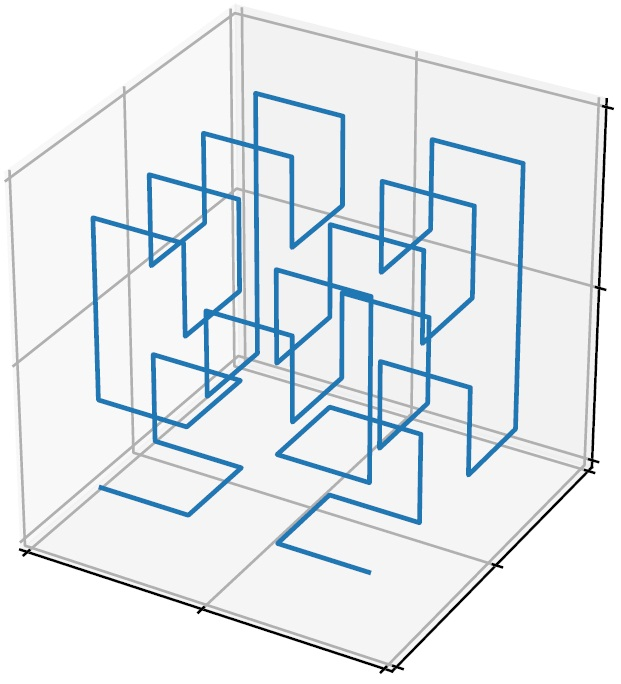
\includegraphics[width=1.0\linewidth]{fig1a.JPG} \\ (a)}
\end{minipage}
\begin{minipage}{0.5\linewidth}
\center{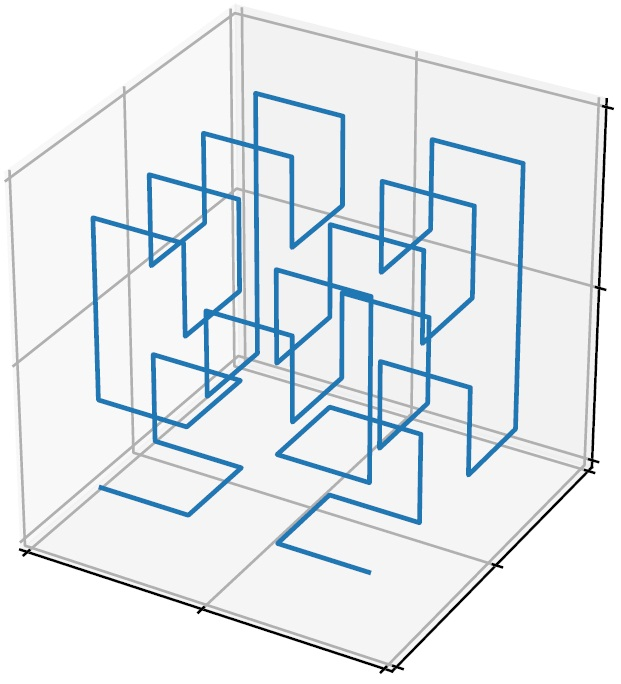
\includegraphics[width=1.0\linewidth]{fig1b.JPG} \\ (b)}
\end{minipage}
\caption{Evolvents in three dimensions with (a) $M=3$ and (b) $M=4$}
\label{evolvents}
\end{figure}


Let us call the process of computing a function value (including the construction of the image $y=y(x)$) as a \textit{trial}, and the pair $\{x, z = \varphi(y(x))\}$ as the outcome of the trial.
When describing a parallel algorithm, we will use the term \textit {iteration} to denote the simultaneous (parallel) execution of several trials (each trial is executed by a separate processor). The number of trials during the $n$-th iteration we will denote as $p$ , and the total number of trials executed during all $n$ iterations as $k(n)$ . In other words, we assume that we have  $p$  processors at our disposal while executing the $n$-th iteration. 

The parallel global search algorithm used in this research (according to \cite{Strongin2000}) can be formulated as follows.
The first $p$ trials are executed at the points $x^0 = 0$, $x^1 = 1$ and at the arbitrary internal points $x^2, ..., x^{p-1}$ of the interval $(0,1)$. Let us assume $n \geq 1$  iterations of the method to be completed, in the course of which the trials in $k=k(n)$ points $x^i, 0 \leq i \leq k,$ have been executed. Then, the points $x^{k+1},...,x^{k+p}$  of the search trials for the next $(n+1)$-th iteration are determined according to the following rules. 

\begin{enumerate}
	\item 
	Renumber the inverse images of all the points from the trials already performed  
\begin{equation}\label{y_i}
y^0=y(x^0), y^1=y(x^1),...,y^k=y(x^k)
\end{equation}
by subscripts in the increasing order of their coordinates, i.e.
\begin{equation}\label{x_i}
0=x_0<x_1<\dots <x_k=1,
\end{equation}
and associate these with the values $z_i=\varphi(y(x_i)), 0\leq i \leq k,$  computed at these points.
\item
Compute the maximum absolute value of the first divided differences
\begin{equation}\label{mu}
\mu = \max_{1 \leq i \leq k}\frac{\left|z_i-z_{i-1}\right|}{\Delta_i},
\end{equation}
where $\Delta_i=\left(x_i-x_{i-1}\right)^{1/N}$. If $\mu = 0$, set $\mu = 1$.
\item
For each interval $(x_{i-1}, x_i), \; 1\leq i \leq k,$  calculate the value
\begin{equation}\label{R}
R(i)=r\mu\Delta_i+\frac{(z_i-z_{i-1})^2}{r\mu\Delta_i}-2(z_i+z_{i-1})
\end{equation}
called the \textit{characteristic} of the interval; the real number $r>1$ being the input parameter of the algorithm.

\item 
Arrange characteristics  $R(i), 1 \leq i \leq k$, in decreasing order 
\begin{equation}\label{Rdec}
R(t_1)\geq R(t_2)\geq \dots \geq R(t_{k})
\end{equation}
and select $p$ largest characteristics with interval numbers $t_j, 1\leq j \leq p$.
\item
Carry out new trials at points $x^{k+j}\in(x_{t_j-1},x_{t_j}), 1\leq j\leq p$, computed according to the formula
\[
x^{k+j} = \frac{x_{t_j}+x_{t_j-1}}{2} - \mathrm{sign}(z_{t_j}-z_{t_j-1})\frac{1}{2r}\left[\frac{\left|z_{t_j}-z_{t_j-1}\right|}{\mu}\right]^N.
\]

\end{enumerate}

The algorithm stops if condition $\Delta_{t_j}<\epsilon$ is satisfied for at least one index $t_j, 1 \leq j \leq p$ ; here $\epsilon>0$ is the predefined accuracy. 
%Также алгоритм останавливается, если превышено заданное при запуске число испытаний $K_{max}$.

The considered variant of the parallelization is \textit{synchronous}, when the transition to the next iteration is performed after full termination of the current one, i.e., after completing the last trial of the current iteration.
% Конкретная реализация данной схемы распараллеливания будет зависеть от архитектуры вычислительной системы, а также от требований к программному обеспечению, необходимому для вычисления значений целевой функции задачи. В данном исследовании проведение испытаний требовало решения жесткой системы ODE (для ее решения был использован метод Radau IIA из бибилиотеки SciPy языка Python). Поэтому распараллеливание было ораганизовано на CPU с использованием технологии MPI. В одном (master) процессе работал алгоритм глобального поиска; остальные (slave) процессы проводили параллельные испытания в рамках выполнения шага 5 алгорита. Объем передаваемых данных между процессами будет небольшим: требуется лишь разослать координаты точек испытаний и затем собрать вычисленные значения целевой функции в этих точках. Одновременно с этим процесс проведения испытания достаточно трудоемкий (время проведения одного испытания занимает не менее 1 сек.), что значительно превышает время передачи данных между процессами. 


\section{Numerical Experiments}\label{Sec_Exp}

The numerical experiments were carried out using the Lobachevsky supercomputer (Lobachevsky State University of Nizhny Novgorod). 
%Указать актуальную конфигурацию
%Each supercomputer node included two quad-core processors Intel Xeon X5570, two NVIDIA Tesla X2070 and 12 Gb RAM.
%Указать актуальное программное обеспечение
%To build the program for running on the Lobachevsky supercomputer, the GCC 4.3.0 compiler, CUDA 6.5 and Intel MPI 2017 were used.
%Для вычисления значений целевой функции задачи использовался Python .

%Parallel global search algorithm запускался со следующими параметрами: параметр надежности $r=3$, точность поиска $\epsilon = 0.01$, плотность построения развертки $m=10$, максимальное число испытаний $K_{max}=1000$. После завершения работы parallel global search algorithm найденное решение уточнялось с помощью локального поиска, использовался Hooke--Jeeves method \cite{HookJeeves}. Точность локального поиска составляла $\epsilon = 0.001$. 

%Далее - описать параллельный запуск и его результаты, например, в виде таблицы с ускорением

%Затем - проинтерпретировать результаты с содержателной точки зрения



\section{Conclusion}

%планы дальнейших работ - реализация метода решения системы 


\medskip

\textbf{Acknowledgments}. This study was supported by the Russian Science Foundation, project No.\,21-11-00204.

%
% ---- Bibliography ----
%
\bibliographystyle{spmpsci}
\bibliography{bibliography}{}

\end{document}
